\documentclass{beamer}
%\usecolortheme{spruce}
\usetheme{A}

\usepackage{amsmath}
\usepackage{datetime}
\usepackage{relsize}
\usepackage{ulem}
\usepackage{amsmath}
\usepackage{calc}
\usepackage{tikz}
\usetikzlibrary{calc}
\usepackage{tabularx}
\usepackage{stmaryrd}
\usepackage{wasysym}
\usepackage{booktabs}
\usepackage{multicol}
\usepackage{colortbl}
\usepackage{tabularx}
\usepackage{centernot}
\usepackage{proof}
\usepackage{graphics}

\definecolor{darkgreen}{HTML}{006400}
\definecolor{darkred}{HTML}{8b0000}
\newcommand{\dg}[1]{\textcolor{darkgreen}{#1}}
\newcommand{\dr}[1]{\textcolor{darkred}{#1}}
\newcommand{\happy}{\dg{\smiley}}
\newcommand{\sad}{\dr{\frownie}}

\newcolumntype{L}{>{\raggedright\arraybackslash}X}
\newcommand{\hnorm}{\vphantom{()}}

\hypersetup{
    colorlinks=true,
    urlcolor=blue,
    pdfpagemode=FullScreen,
}

\newcommand{\li}{%
	\scalebox{1}[1]{$\multimap$}
}
\newcommand{\prop}[1]{%
	\ensuremath{#1}%
}
\newcommand{\term}[1]{%
	\ensuremath{\mathsf{#1}}%
}


\begin{document}



\date{Logic for the AI Spring\\
September 2022, Como}

\title[]{Neurosymbolic Proof Search\\
for Linguistics}
\author{%
    Konstantinos Kogkalidis
    \inst{Utrecht Institute of Linguistics OTS, Utrecht University}
}


{%
\setbeamertemplate{headline}{}
\frame{\titlepage
\hspace{-10pt}
\begin{minipage}{0.5\textwidth}
\begin{minipage}{0.35\textwidth}

\includegraphics[scale=0.065]{NWO logo - RGB_wit_rondom_0.jpg}%
\end{minipage}%
\begin{minipage}{0.65\textwidth}
\smaller[3]
\centering
A composition calculus for vector-based semantic modelling
with a localization for Dutch\\~\\
NWO 360-89-070, 2017-2022
\end{minipage}
\end{minipage}%
\hfill
\begin{minipage}{0.45\textwidth}
\hfill
\raisebox{-5.5pt}{
\includegraphics[scale=0.5]{UU_logo_2021_EN_RGB.jpg}}
\end{minipage}%
}
}

\section{Background}

\begin{frame}{The Holy Trinity}
	\smaller	
	
	\begin{tabularx}{1\textwidth}{@{}ccc@{}}
		\toprule
		\textbf{Language}			& \textbf{Logic}			& \textbf{Computation}\\
		\toprule
		grammars					& substructural logics 		& $\lambda$-calculi\\
		empirical linguistic rules & logical inference rules 	& computation steps\\
		grammaticality				& provability				& type inhabitation\\
		sentence					& proof						& program
	\end{tabularx}\vfill
	
	\uncover<2->{
	\textbf{Lexicon}: a look-up table from words to \textit{types} and \textit{meanings}\vfill
	
	\uncover<3->{
	\alt<4->{
		A \textbf{heretical} perspective:
		\begin{itemize}
			\item focus on \textit{deep} (discontinuous) syntax
			\item use ILL as core logic (linear types)
			\item $\diamondsuit$, $\Box$ modalities for dependency annotation
			\item extra semantic dimension: adjunct/complement distinction
		\end{itemize}
	}
	{
		The \textbf{type-logical} perspective:
		\begin{itemize}
			\item focus on \textit{surface} syntax
			\item use LC/NL as core logic (ordered \& linear types)
			\item $\diamondsuit$, $\Box$ modalities for structural control
			\item applicative derivational semantics via proof/term morphisms
		\end{itemize}
	}
	}}
\end{frame}

\section{Heresy}
\begin{frame}{Types}
	\smaller	
	ILL$_{\li}$ plus $\diamondsuit, \Box$ modalities for \textit{dependency domain demarcation}.
	\vfill
		
	$\mathbb{T}$ inductively defined as:
	\[
		\mathbb{T} := A \ 
					\uncover<2->{| \  T \li T \ 
					\uncover<3->{| \ \diamondsuit^d  T \ 
					\uncover<4->{| \ \Box^d T
					}}}
					\qquad A \in \mathbb{A}, T \in \mathbb{T}
	\]
	\vfill	

	\begin{itemize}
		\item[$\mathbb{A}$] 				-- closed set of base types
		\uncover<2->{
		\item[$\li$]						-- linear function builder
		\uncover<3->{
		\item[$\diamondsuit$] 				-- reserved for "necessary arguments", i.e. complements
		\uncover<4->{
		\item[$\Box$]						-- reserved for "optional functors", i.e. adjuncts
		}}}
	\end{itemize}
\end{frame}

\begin{frame}{Terms}
\smaller

\renewcommand{\arraystretch}{1.15}
{
\begin{tabularx}{\textwidth}{@{}c@{\qquad}c@{}}
$\infer[Lex]{\term{c}: T \vdash \term{c}: T}{\vphantom{T}}$
&
\uncover<2->{
$\infer[\li E]{\Gamma, \Delta \vdash \term{s\ t}: T_2}{\Gamma \vdash \term{s}: T_1 \li T_2 & \Delta \vdash \term{t}: T_1}$}
\\
\\
\uncover<3->{
$\infer[\diamondsuit^d I]{\langle \Gamma \rangle^{d} \vdash \vartriangle^d \term{t}: \diamondsuit^d T}{\Gamma \vdash \term{t}: T}$
}
&
\uncover<4->{
$\infer[\Box^d E]{\langle \Gamma \rangle^d \vdash \blacktriangledown^d \term{s}: T}{\Gamma \vdash \term{s}: \Box^d T}$}
\\
\\
\textcolor{gray!30}{
$\infer[Ax]{\term{x}: T \vdash \term{x}: T}	{\vphantom{T}}$}
&
\textcolor{gray!30}{
$\infer[\li I]{\Gamma \vdash \lambda\term{x.s}: T_1 \li T_2}{\Gamma, \term{x}: T_1 \vdash \term{s}: T_2}$}
\\
\\
\textcolor{gray!30}{
$\infer[\Box^d I]{\Gamma \vdash \blacktriangle^d \term{s}: \Box^d T}{\langle \Gamma \rangle^d \vdash \term{s}: T}$}
&
\textcolor{gray!30}{
$\infer[\diamondsuit^d E]{\Gamma[\Delta] \vdash \term{t}[\term{x} \mapsto \triangledown^d \term{s}]: T_2}{
		\Gamma[\langle \term{x}: T_1 \rangle^d] \vdash \term{t}: T_2			
		&\quad
		\Delta \vdash \term{s}: \diamondsuit^d T_1}$
}
\\
\\
\multicolumn{2}{c}{
\textcolor{gray!30}{
$\infer[\mathsf{X}]{\langle\Gamma, \Delta\rangle^d,  \langle \term{x}: T_1 \rangle^\mathsf{X} \vdash \term{s}: T_2}{
\langle\Gamma, \langle \term{x}: T_1 \rangle^\mathsf{X}, \Delta\rangle^d \vdash \term{s}: T_2}$}}
\end{tabularx}}
\end{frame}

\newcommand{\cnj}{\diamondsuit^{cnj}}
\newcommand{\obj}{\diamondsuit^{obj}}
\newcommand{\md}{\Box^{mod}}

\begin{frame}{Example}
	
	\begin{center}
		\smaller[2]
		``Meloni e Salvini in Piazzale Loreto''
	\end{center}
	
	\smaller[4]
	\[
		\infer[\hspace{-3.5pt}\li E]{
		\langle \term{c_3}, \langle \langle \term{c_5} \rangle^{app}, \term{c_4}\rangle^{obj} \rangle^{mod},\term{c_1}, \langle \term{c_0} \rangle^{cnj}, \langle \term{c_2} \rangle^{cnj} \vdash \prop{np}
		}{
			\infer[\hspace{-3.5pt}\Box E]{\langle \term{c_3}, \langle \langle \term{c_5} \rangle^{app}, \term{c_4}\rangle^{obj} \rangle^{mod} \vdash \prop{np}\li\prop{np}}{
				\infer[\hspace{-3.5pt}\li E]{\term{c_3}, \langle \langle \term{c_5} \rangle^{app}, \term{c_4}\rangle^{obj} \vdash \md(\prop{np}\li\prop{np})}{
					\hspace{-15pt}\infer{\term{c_3} \vdash \obj\prop{np}\li\md(\prop{np}\li\prop{np})}{
						\term{c_3}: \term{in}
					}
					&
					\hspace{-12pt}\infer[\hspace{-3.5pt}\diamondsuit I]{\langle \langle \term{c_5} \rangle^{app}, \term{c_4}\rangle^{obj} \vdash \obj\prop{np}}{
						\infer[\hspace{-3.5pt}\li E]{\langle \term{c_5} \rangle^{app}, \term{c_4} \vdash \prop{np}}{
							\infer[\hspace{-3.5pt}\Box E]{\langle\term{c_5}\rangle^{app} \vdash \prop{np}\li\prop{np}}{
								\infer{\term{c_5} \vdash \Box^{app}(\prop{np}\li\prop{np})}{
									\term{c_5}: \term{Loreto}
								}
							}
							&
							\infer{\term{c_4} \vdash \prop{np}}{\term{c_4}: \term{Piazzale}}
						}
					}
				}
			}
			&
			\hspace{-10pt}\infer[\hspace{-3.5pt}\li E]{\term{c_1}, \langle \term{c_0} \rangle^{cnj}, \langle \term{c_2} \rangle^{cnj} \vdash \prop{np}}{
					\infer{\term{c_1} \vdash \cnj\prop{np} \li \cnj\prop{np} \li \prop{np}}{
						\term{c_1}: \term{e}
					}
					&
					\infer[\hspace{-3.5pt}\diamondsuit I]{\langle \term{c_0}\rangle^{cnj}\vdash \cnj\prop{np}}{
							\infer{\term{c_0} \vdash \prop{np}}{\term{c_0}: \term{Meloni}}
					}
				&
				\infer[\hspace{-3.5pt}\diamondsuit I]{\langle \term{c_2}\rangle^{cnj}\vdash \cnj\prop{np}}{
					\infer{\term{c_0} \vdash \prop{np}}{\term{c_2}: \term{Salvini}}
				}
			}
		}
	\]
	\larger[3]
	$\lambda$ read-off:
	\smaller
	\[
		\blacktriangledown^{mod}(
			\term{in}~(\blacktriangledown^{app}\!(\term{Loreto})~\term{Piazzale})
		)
		~
		(
		\term{e}~\vartriangle^{cnj}\!(\term{Meloni})
		~\vartriangle^{cnj}\!(\term{Salvini})
		)
	\]
	\vfill
	\flushright	\textbf{Resource}: \ae thel $\sim$70\,000 proofs (in Dutch)\\
	see: abs/1912.12635
	\vspace{-10pt}
\end{frame}

\begin{frame}{Towards Wide Coverage}
	\smaller
	\textbf{Lexical Types on demand?}\\
	\begin{tabularx}{1\textwidth}{@{}l@{$\implies$}l@{}}
	Word $\mapsto$ Type is not 1-1 & how to choose right type?\\
	Corpus $\subset$ language & new words?\\
	Inductive type universe & new types?
	\end{tabularx}\\[15pt]

	\textbf{Proof Search?}\\
	\begin{tabularx}{1\textwidth}{@{}l@{$\implies$}l@{}}
	Non-directional types & all permutations must be considered\\
	Hypothetical reasoning & Prawitz problem
	\end{tabularx}
\end{frame}

\section{Neural}
\newcommand{\vnorm}[1]{%
	\ensuremath{\vphantom{\diamondsuit^X}{#1}}%
}
\newcommand{\qmarkat}[2]{\alt<#1>{#2}{\vnorm{???}}}
\newcommand{\rqmarkat}[3]{\alt<#1>{\qmarkat{#2}{\dr{\vnorm{#3}}}}{}}
\newcommand{\gqmarkat}[3]{\alt<#1>{\qmarkat{#2}{\dg{\vnorm{#3}}}}{}}

\begin{frame}{Contextual Dynamic Types}
	\smaller[2]
	
	\centering
	\begin{tikzpicture}[every node/.style={outer sep=0pt},
						tagger/.style={rectangle, inner sep=0pt, minimum width=330pt, minimum height=20pt, rounded corners, very thick, draw=black, fill=gray!20}]
		%%%%%%%%%%%%%%%%%%%%%%%%%%%%%%%%%%%%%%%%%%%%%%%%%%%%%%%%%%%%%%%%%%%%%%%%%
		% moving box
		\visible<2>{
		\node[tagger] 	(tagger)		at (5.25, 0.5)					{};
		}
		\visible<3>{
		\node[tagger] 	(tagger)		at (5.25, 1.3)					{};
		}
		\visible<4>{
		\node[tagger] 	(tagger)		at (5.25, 2.1)					{};
		}
		\visible<5>{
		\node[tagger] 	(tagger)		at (5.25, 2.8)					{};
		}
		%%%%%%%%%%%%%%%%%%%%%%%%%%%%%%%%%%%%%%%%%%%%%%%%%%%%%%%%%%%%%%%%%%%%%%%%%
		% word sequence
		\node			(Meloni)		at (0, 0)					{Meloni};
		\node			(e)				at (1.8, 0)					{e};
		\node			(Salvin)		at (3.6, 0)					{Salvini};
		\node			(in)			at (5.2, 0)					{in};
		\node			(Piazzale)		at (7.0, 0)					{Piazzale};
		\node			(Loreto)		at (8.8, 0)					{Loreto};
		%%%%%%%%%%%%%%%%%%%%%%%%%%%%%%%%%%%%%%%%%%%%%%%%%%%%%%%%%%%%%%%%%%%%%%%%%
		% formula trees
		\node			(w1_np)			at (0, 0.5)					{\gqmarkat{1-}{2-}{\prop{np}}};
		%
		\node			(w2_li1)		at (1.8, 0.5)				{\gqmarkat{1-}{2-}{\li}};
		\node			(w2_c1)			at (1.2, 1.3)				{\rqmarkat{2-}{3-}{\cnj}};
		\node			(w2_np1)		at (1.2, 2.1)				{\rqmarkat{3-}{4-}{\prop{np}}};
		\node			(w2_li2)		at (2.4, 1.3)				{\gqmarkat{2-}{3-}{\li}};
		\node			(w2_c2)			at (2.0, 2.1)				{\rqmarkat{3-}{4-}{\cnj}};
		\node			(w2_np2)		at (2.0, 2.8)				{\rqmarkat{4-}{5-}{\prop{np}}};
		\node			(w2_np3)		at (2.8, 2.1)				{\gqmarkat{3-}{4-}{\prop{np}}};
		\visible<2->{
		\draw (w2_li1) -- (w2_c1);
		\draw (w2_li1) -- (w2_li2);
		}
		\visible<3->{
		\draw (w2_c1) -- (w2_np1);
		\draw (w2_li2) -- (w2_c2);
		\draw (w2_li2) -- (w2_np3);
		}
		\visible<4->{
		\draw (w2_c2) -- (w2_np2);}
		%
		\node			(w3_np)			at (3.6, 0.5)				{\gqmarkat{1-}{2-}{\prop{np}}};
		%
		\node			(w4_li1)		at (5.2, 0.5)				{\gqmarkat{1-}{2-}{\li}};
		\node			(w4_mod)		at (5.8, 1.3)				{\gqmarkat{2-}{3-}{\md}};
		\node			(w4_obj)		at (4.6, 1.3)				{\rqmarkat{2-}{3-}{\obj}};
		\node			(w4_np1)		at (4.6, 2.1)				{\rqmarkat{3-}{4-}{\prop{np}}};
		\node			(w4_li2)		at (5.8, 2.1)				{\gqmarkat{3-}{4-}{\li}};
		\node			(w4_np2)		at (5.4, 2.8)				{\rqmarkat{4-}{5-}{\prop{np}}};
		\node			(w4_np3)		at (6.2, 2.8)				{\gqmarkat{4-}{5-}{\prop{np}}};
		\visible<2->{
		\draw (w4_li1) -- (w4_mod);
		\draw (w4_li1) -- (w4_obj);
		}
		\visible<3->{
		\draw (w4_obj) -- (w4_np1);
		\draw (w4_mod) -- (w4_li2);
		}
		\visible<4->{
		\draw (w4_li2) -- (w4_np2);
		\draw (w4_li2) -- (w4_np3);
		}
		%
		\node			(w5_np)			at (7, 0.5)					{\gqmarkat{1-}{2-}{\prop{np}}};
		%
		\node			(w6_app)		at (8.8, 0.5)				{\gqmarkat{1-}{2-}{\Box^{app}}};
		\node			(w6_li)			at (8.8, 1.3)				{\gqmarkat{2-}{3-}{\li}};
		\node			(w6_np1)		at (8.4, 2.1)				{\rqmarkat{3-}{4-}{\prop{np}}};
		\node			(w6_np2)		at (9.2, 2.1)				{\gqmarkat{3-}{4-}{\prop{np}}};
		\visible<2->{
		\draw (w6_app) -- (w6_li);
		}
		\visible<3->{
		\draw (w6_li) -- (w6_np1);
		\draw (w6_li) -- (w6_np2);
		}
		%
		\node			(dash)			at (10, 0.5)				{\vnorm{\vdash}};
		\node			(conc)			at (10.6, 0.5)				{\rqmarkat{1-}{2-}{\prop{np}}};
	\end{tikzpicture}
	\vfill
	\visible<6>{
	\flushright{
	gray box := heterogenous graph convolution kernel\\
	see: abs/2203.12235
	}}
\end{frame}



\begin{frame}{Proofs as \alt<2->{Neural}{} Graphs}
	\smaller[2]

	\vspace{5pt}
	\begin{minipage}[t][30pt]{1\textwidth}
	\alt<2->{
		\textbf{The problem}\\
		Find bijection $\dg{ \{p: A^{+} \}} \longleftrightarrow \dr{\{ n: A^{-} \}}~ \forall ~ A \in \mathbb{A}$ in sentence
	
		\hfill \textit{here} $\{\dg{1} \mapsto \dr{2},~ \dg{4} \mapsto \dr{7},~ \dg{5} \mapsto \dr{3},~ \dg{8} \mapsto \dr{12},~ \dg{9} \mapsto \dr{10},~ \dg{11} \mapsto \dr{6}\}$
		
		\visible<3->{
		\textbf{The solution}\\
		 compute \& normalize $\dg{A^{+}} \times \dr{A^{-}}$, train against underlying permutation matrix\\
		}
	}{
		\textbf{From N.D. to Proof Nets}
		\begin{itemize}
			\item proof structure : tree $\to$ graph
			\item proof construction : depth induction $\to$ parallel assignment
			\item proof search : backward/forward chaining $\to$ factorial combinatorics
		\end{itemize}
	}
	\end{minipage}\vspace{30pt}
	\begin{minipage}[t][200pt]{1\textwidth}
	\alt<3->{
		\centering
		\hfill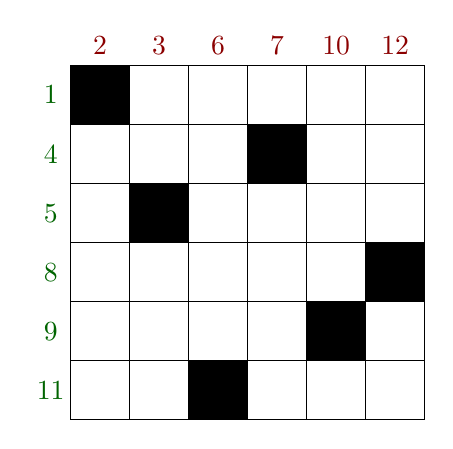
\begin{tikzpicture}
			\draw[step=0.75] (0,0) grid (4.5,4.5);
			\node (1) 	at	(-0.25, 4.125)	{\dg{1}};
			\node (4)	at	(-0.25, 3.375)	{\dg{4}};
			\node (5)	at 	(-0.25, 2.625)	{\dg{5}};
			\node (8)	at 	(-0.25, 1.875)	{\dg{8}};
			\node (9)	at 	(-0.25, 1.125)	{\dg{9}};
			\node (11)	at 	(-0.25, 0.375)	{\dg{11}};
			%
			\node (2)	at 	(0.375, 4.75)	{\dr{2}};
			\node (3)	at 	(1.125, 4.75)	{\dr{3}};
			\node (6)	at 	(1.875, 4.75)	{\dr{6}};
			\node (7)	at 	(2.625, 4.75)	{\dr{7}};
			\node (10)	at 	(3.375, 4.75)	{\dr{10}};
			\node (12)	at  (4.125, 4.75)	{\dr{12}};
			%
		   	\fill[black]	(0, 3.75) 		rectangle +(0.75, 0.75);
		   	\fill[black]	(2.25, 3)		rectangle +(0.75, 0.75);
		   	\fill[black]	(0.75, 2.25)	rectangle +(0.75, 0.75);
		   	\fill[black]	(3.75, 1.5)		rectangle +(0.75, 0.75);
		   	\fill[black]	(3, 0.75)		rectangle +(0.75, 0.75);
		   	\fill[black]	(1.5, 0)		rectangle +(0.75, 0.75);
		\end{tikzpicture}%
		\hfill	see: abs/2009.12702
	}{
		\centering
		\begin{tikzpicture}[every node/.style={outer sep=0pt}]
			%%%%%%%%%%%%%%%%%%%%%%%%%%%%%%%%%%%%%%%%%%%%%%%%%%%%%%%%%%%%%%%%%%%%%%%%%
			% word sequence
			\node			(Meloni)		at (0, 0)					{Meloni};
			\node			(e)				at (1.8, 0)					{e};
			\node			(Salvin)		at (3.6, 0)					{Salvini};
			\node			(in)			at (5.2, 0)					{in};
			\node			(Piazzale)		at (7.0, 0)					{Piazzale};
			\node			(Loreto)		at (8.8, 0)					{Loreto};
			%%%%%%%%%%%%%%%%%%%%%%%%%%%%%%%%%%%%%%%%%%%%%%%%%%%%%%%%%%%%%%%%%%%%%%%%%
			% formula trees
			\node			(w1_np)			at (0, 0.5)					{\gqmarkat{1-}{1-}{\prop{1}}};
			%
			\node			(w2_li1)		at (1.8, 0.5)				{\gqmarkat{1-}{1-}{\li}};
			\node			(w2_c1)			at (1.2, 1.3)				{\rqmarkat{1-}{1-}{\cnj}};
			\node			(w2_np1)		at (1.2, 2.1)				{\rqmarkat{1-}{1-}{\prop{2}}};
			\node			(w2_li2)		at (2.4, 1.3)				{\gqmarkat{1-}{1-}{\li}};
			\node			(w2_c2)			at (2.0, 2.1)				{\rqmarkat{1-}{1-}{\cnj}};
			\node			(w2_np2)		at (2.0, 2.8)				{\rqmarkat{1-}{1-}{\prop{3}}};
			\node			(w2_np3)		at (2.8, 2.1)				{\gqmarkat{1-}{1-}{\prop{4}}};
			\draw (w2_li1) -- (w2_c1);
			\draw (w2_li1) -- (w2_li2);
			\draw (w2_c1) -- (w2_np1);
			\draw (w2_li2) -- (w2_c2);
			\draw (w2_li2) -- (w2_np3);
			\draw (w2_c2) -- (w2_np2);
			%
			\node			(w3_np)			at (3.6, 0.5)				{\gqmarkat{1-}{1-}{\prop{5}}};
			%
			\node			(w4_li1)		at (5.2, 0.5)				{\gqmarkat{1-}{1-}{\li}};
			\node			(w4_mod)		at (5.8, 1.3)				{\gqmarkat{1-}{1-}{\md}};
			\node			(w4_obj)		at (4.6, 1.3)				{\rqmarkat{1-}{1-}{\obj}};
			\node			(w4_np1)		at (4.6, 2.1)				{\rqmarkat{1-}{1-}{\prop{6}}};
			\node			(w4_li2)		at (5.8, 2.1)				{\gqmarkat{1-}{1-}{\li}};
			\node			(w4_np2)		at (5.4, 2.8)				{\rqmarkat{1-}{1-}{\prop{7}}};
			\node			(w4_np3)		at (6.2, 2.8)				{\gqmarkat{1-}{1-}{\prop{8}}};
			\draw (w4_li1) -- (w4_mod);
			\draw (w4_li1) -- (w4_obj);
			\draw (w4_obj) -- (w4_np1);
			\draw (w4_mod) -- (w4_li2);
			\draw (w4_li2) -- (w4_np2);
			\draw (w4_li2) -- (w4_np3);
			%
			\node			(w5_np)			at (7, 0.5)					{\gqmarkat{1-}{1-}{\prop{9}}};
			%
			\node			(w6_app)		at (8.8, 0.5)				{\gqmarkat{1-}{1-}{\Box^{app}}};
			\node			(w6_li)			at (8.8, 1.3)				{\gqmarkat{1-}{1-}{\li}};
			\node			(w6_np1)		at (8.4, 2.1)				{\rqmarkat{1-}{1-}{\prop{10}}};
			\node			(w6_np2)		at (9.2, 2.1)				{\gqmarkat{1-}{1-}{\prop{11}}};
			\draw (w6_app) -- (w6_li);
			\draw (w6_li) -- (w6_np1);
			\draw (w6_li) -- (w6_np2);
			%
			\node			(dash)			at (10, 0.5)				{\vnorm{\vdash}};
			\node			(conc)			at (10.6, 0.5)				{\rqmarkat{1-}{1-}{\prop{12}}};
			%%%%%%%%%%%%%%%%%%%%%%%%%%%%%%%%%%%%%%%%%%%%%%%%%%%%%%%%%%%%%%%%%%%%%%%%%
			% axiom links
			\draw[->] (w1_np) -- ($(w1_np) + (0, 2.25)$) -| (w2_np1);
			\draw[->] (w3_np) -- ($(w3_np) + (0, 3)$) -| (w2_np2);
			\draw[->] (w2_np3) -- ($(w2_np3) + (0, 1.75)$) -| (w4_np2);
			\draw[->] (w5_np) -- ($(w5_np) + (0, 2.25)$) -| (w6_np1);
			\draw[->] (w4_np3) -- ($(w4_np3) + (0, 1)$) -| (conc);
			\draw[->] (w6_np2) -- ($(w6_np2) + (0, 1.25)$) -| (w4_np1);
		\end{tikzpicture}
		}
	\end{minipage}
\end{frame}

\section{TLDR}


\begin{frame}{Final words}
	\smaller
	\dg{done}
	\begin{itemize}
		\item a logic for dependency control
		\item a corpus of linguistically grounded theorems
		\item a hyper-efficient neurosymbolic parser
	\end{itemize}
	\vfill
	
	\uncover<2->{
	\dr{todo}
	\begin{itemize}
		\item derivational ambiguity?
		\uncover<3->{\item neural integration of proof verification?
		\uncover<4->{\item neural proof semantics?
		\uncover<5->{\item adaptation to other languages/frameworks?
		\uncover<6->{\item thank audience
		}}}}
	\end{itemize}
	}
\end{frame}

\end{document}